\documentclass{article}
\usepackage{amsmath}
\usepackage[utf8]{inputenc}
\usepackage{natbib}
\usepackage{graphicx}

\title{LELEC2103:Labview4}
\author{Bronchain Olivier \\ Schellekens Vincent}
\date{\today}

\begin{document}
\maketitle

\section{Pre-Lab}
    \subsection{Toeplitz}
        The metode impletemented for the Toeplitz matrix takes 2 vectors as input. The first one $x[m]$ ( $0\le m \le M-1$) decribes first row of the matrix and the second one $y[n]$ ($0 \le n \le N-1$) describes the column of the matrix. The Toeplitz matrix is given by the Equation \ref{toeplitz}.
        \begin{equation}
            Toeplitz(x,m) =
                \begin{pmatrix} 
                    x[0] & x[1] & \cdots& \cdots & x[M-2] & x[M-1] \\
                    y[1] & x[0] & x[1] & \cdots & x[M-2] & x[M-2] \\
                    \vdots & \ddots & \ddots & \ddots & \ddots & \vdots \\
                    y[N-1] & \cdots &  & & & \\
                \end{pmatrix}
                \label{toeplitz}
        \end{equation}
        A problem occurs if $x[0]!=y[0]$ because those elements should be the same. A solution in the implementation is to return an error when those values are different. In practice our implemetnation just takes the value of the row (x).
        
    \subsection{Influence of equalizer length}
        The goal of this is to find a filter $f_{nd}$ (equalize) of length $L_g$ to apply to the received signal $y[n]$ such that $f_{nd}$ will cancel the action of the canal on the signal ($h[n]$). The goal is then to find a filter such that:
            \begin{equation}
                \sum_{l=0}^{L_f} f[l]\hat{h}[n-l] \cong \delta[n-n_d]
            \end{equation}  
            
        where $\hat{h}$ is the estimated chanel and $L_f$ the equalizer length. We espect that the convolution of those filters will give a $\delta$. Because we suppose that $h$ have a finite length we need a $f_{nd}$ of infinite length. Figures \ref{1-3} and \ref{4-6} show the evolution of the constaletion as function the equalizer length $L_f$. We observe that when $L_f$ grows, the constellation is better. In fact the equalizer $f_{nd}$ get more points to cancel the chanel $h$. 
    \begin{figure}[h]
        \centering
        \begin{tabular}{ccc}
            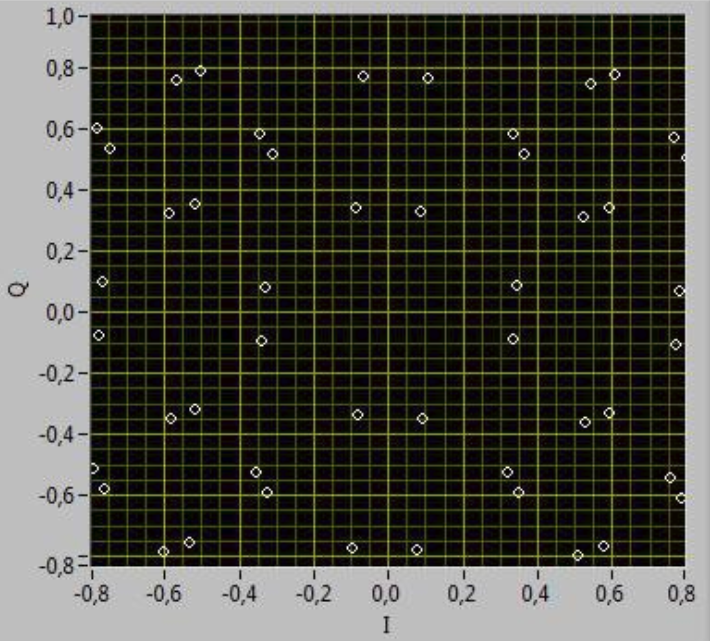
\includegraphics[width= 0.3 \textwidth]{eq1.png} & 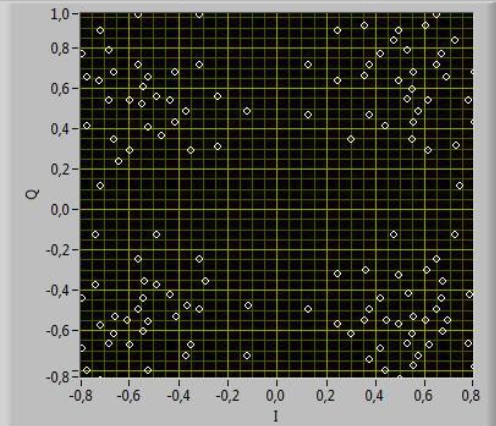
\includegraphics[width= 0.3 \textwidth]{eq2.png} & 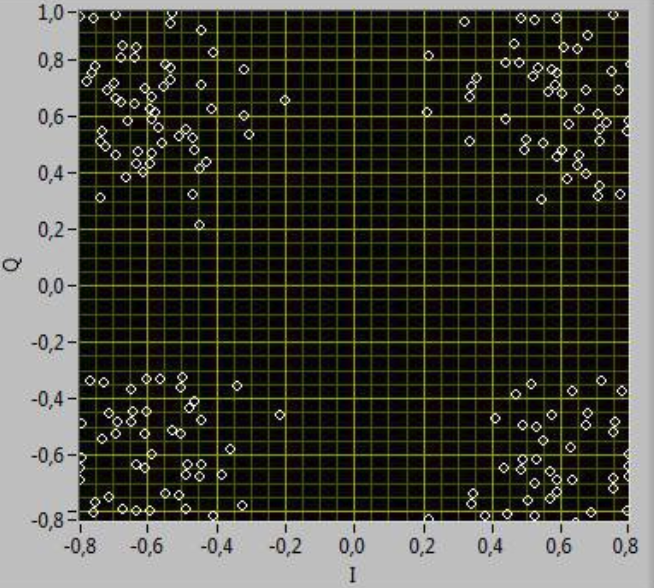
\includegraphics[width= 0.3 \textwidth]{eq3.png} \\
        \end{tabular}
        \caption{Constalation for equalize length from 1 to 3 \label{1-3}}.
    \end{figure}
    \begin{figure}[h]
        \centering
        \begin{tabular}{ccc}
            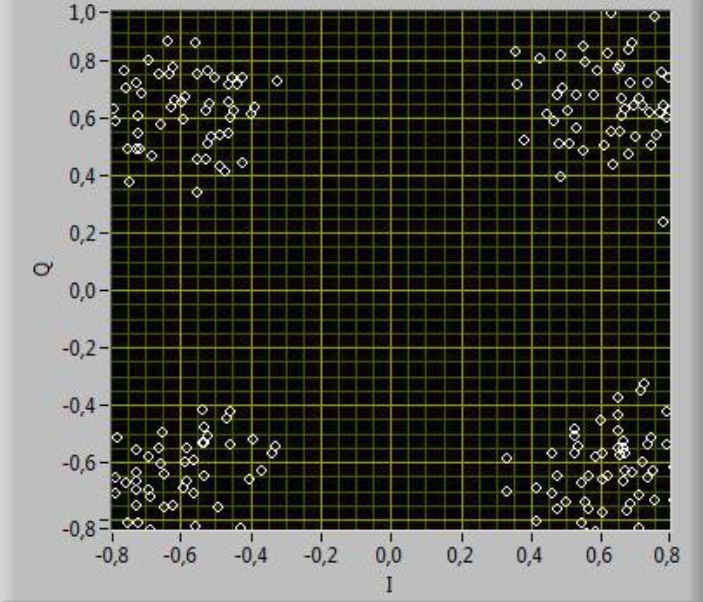
\includegraphics[width= 0.3 \textwidth]{eq4.png} & 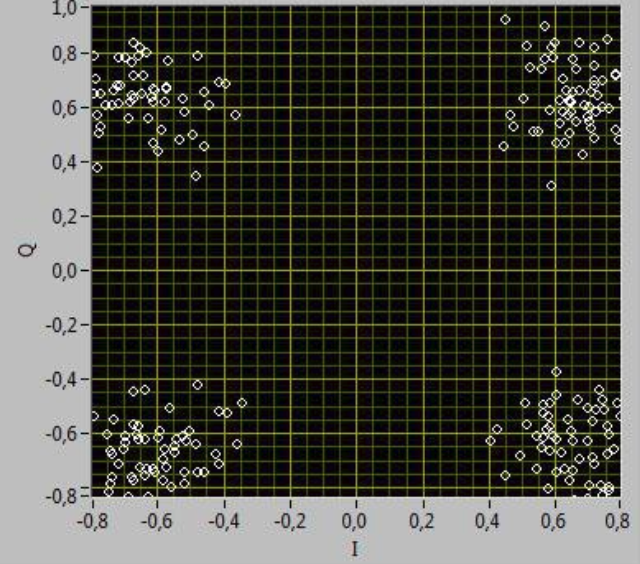
\includegraphics[width= 0.3 \textwidth]{eq5.png} & 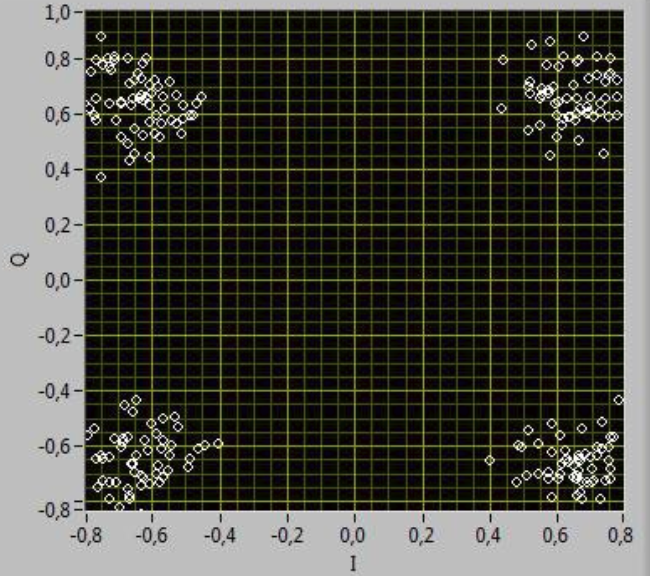
\includegraphics[width= 0.3 \textwidth]{eq6.png} \\
        \end{tabular}
        \caption{Constalation for equalize length from 4 to 6 \label{4-6}}.
    \end{figure}
    
    \subsection{Influence of noise}
    The figure \ref{snr1} shows the average BER with respect to the SNR for two different equalizer lengths. We can see that for high SNR values, the longest equalizer gives the least errors, but if the SNR is low (close to 1) the longest equalizer is less performant. This must be due to the fact that noise is corrupting the training sequence, therefore corrupting the equalizing filter, and afterwards the corrupted filter corrupts the symbols even more. In the case of a simple AWGN channel, the BER is always lower (because the channel is - apart from the noise - ideal) even if the equalizer length is 1.
    
    \begin{figure}[h!]
    \centering
    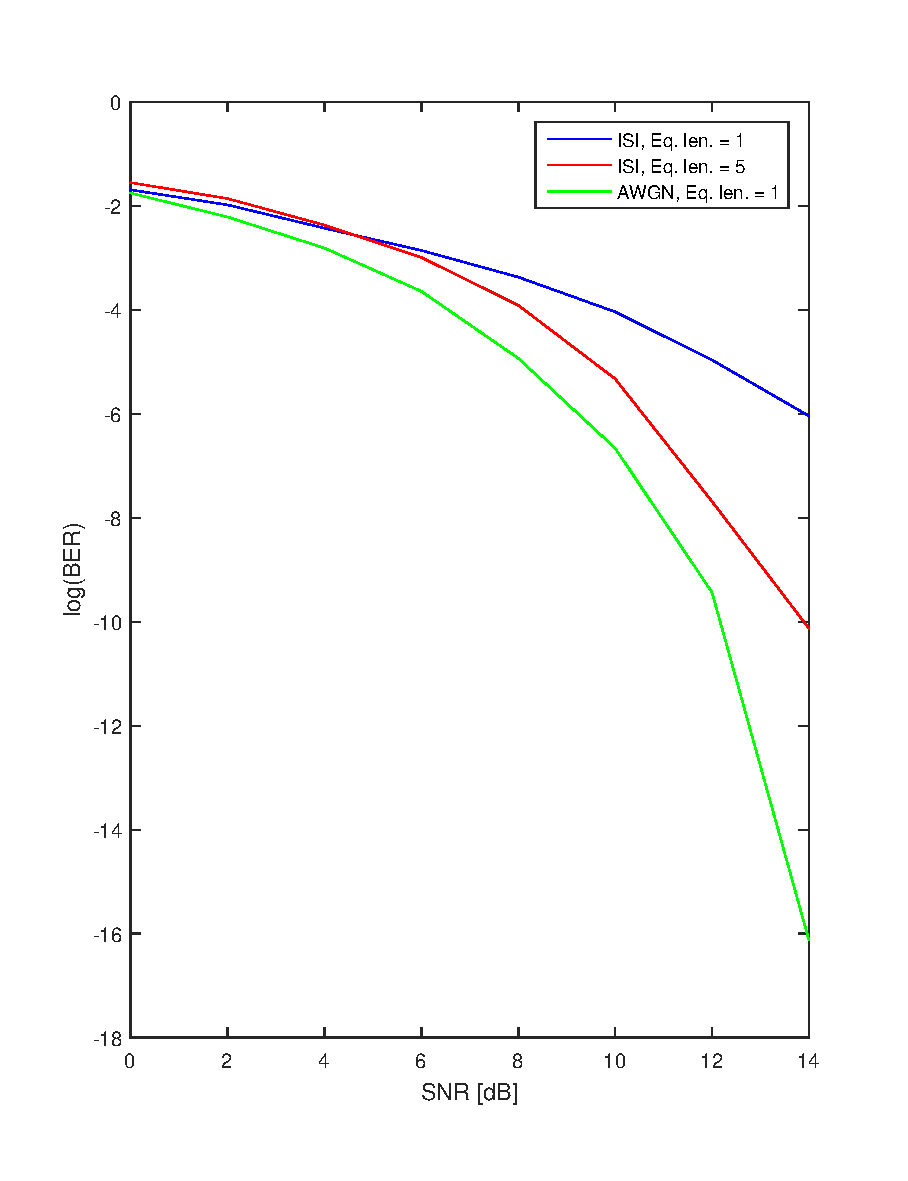
\includegraphics[scale = 0.6]{SNR1}
    \caption{Different BER versus SNR plots. In blue, the ISI channel with equalizer length 1.  In red, the ISI channel with equalizer length 5.  In green, the AWGN channel with equalizer length 1.}
    \label{snr1}
\end{figure}
    
\section{Lab}
\subsection{Narrowband channel}
Here we observe the constellation before the equalization, to see the impact of the channel on the constellation. The symbol rate is $100k [symbols/s]$ and the bandwith of the channel is $144MHz$. %????

    With those value, the Symbol rate is equal to $10M$.The symbol periode is then $1/10M = 0.1\mu s$.

Figures \ref{con1} and \ref{con2} show the influence of the channel on the constellations. We can see two main effects. First, the modulus of the complex symbols is affected, as the channel attenuates the signal. This attenuation is, as can be seen in the figures, variable. The second effect of the channel without equalizer is to add a variable phase shift to the complex symbols. This is problematic because it means the symbols get mixed up if we don't fix this phase shift with the equalizer.

\begin{figure}[h!]
    \centering
    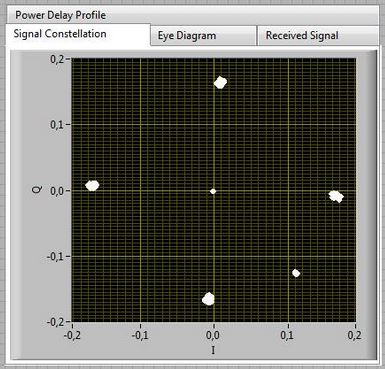
\includegraphics[scale = 0.6]{con1}
    \caption{Received constellation without equalizer (1).}
    \label{con1}
\end{figure}

\begin{figure}[h!]
    \centering
    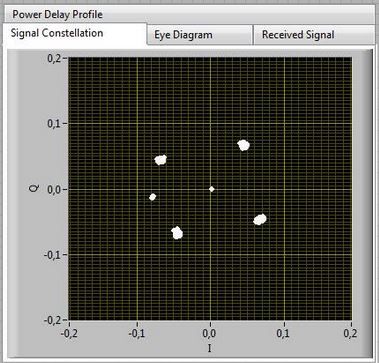
\includegraphics[scale = 0.6]{con2}
    \caption{Received constellation without equalizer (2).}
    \label{con2}
\end{figure}


\subsection{Wideband channel}
    With those value, the Symbol rate is equal to $0.1M$.The symbol periode is then $1/0.1M = 10\mu s$.
\subsubsection{Bandwidth}
    During this experiment, the channel bandwidth was equal to $4E+7$. Figure \ref{chanel} shows the channel response. We observe that this response is close to a $\delta$. This is a due to the wideband. In fact a large band in frequency domain give a short delta in the temporal domain.
    \begin{figure}[h!]
        \centering
        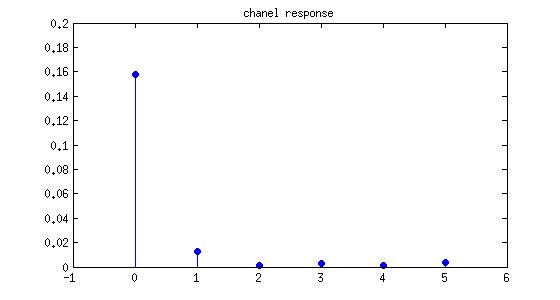
\includegraphics[width = 0.8 \textwidth]{chanel.jpg}
        \caption{Estimate chanel response $h[n]$\label{chanel}}
    \end{figure}
    
\subsubsection{Power-delay}
    The power-delay is given by Equation \ref{powConti} in continuous time and by Equation \ref{powDisc} in discrete time. $h(t)$ is the channel response and $\hat{h}[n]$ is the estimated response. This can be observe in Figure \ref{delay}. There is a heavy link with Figure \ref{chanel}. The conclusion are the same. We observe that the response is close to a $\delta$.  
     \begin{equation}
        P(\delta)=E{|h(\delta)|^2}
        \label{powConti}
     \end{equation}
     \begin{equation}
        P[n] = E{|\hat{h}[n]|^2}
        \label{powDisc}
     \end{equation}
     
     \begin{figure}[h!]
        \centering
        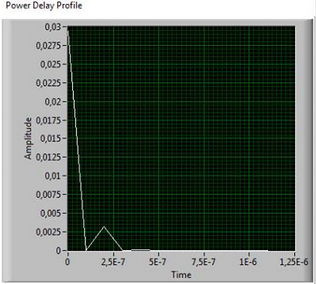
\includegraphics[width=0.5\textwidth]{powerdelay.png}
        \caption{Power-delay of the channel $P(\delta)$ \label{delay}}
     \end{figure}
    \begin{figure}[h!]
        \centering
        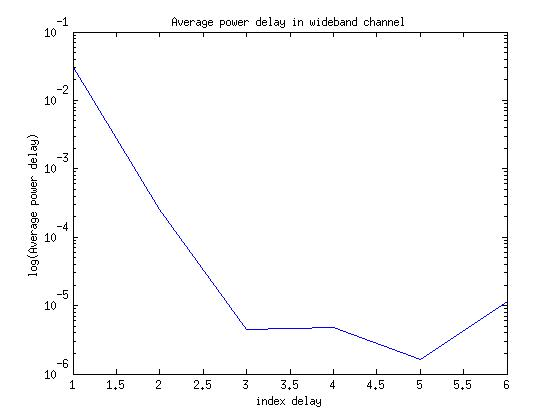
\includegraphics[width = 0.7 \textwidth]{average.jpg}
        \caption{Average power delay in log scale \label{av}}
    \end{figure}

\section{Lab turn in}
If the channel $h(\tau)$ has nonzero support for $\tau \in [0,2.5\mu s]$, and the symbol period is $T_s$, the number of nonzero taps is $\frac{2.5\mu s}{T_s}$, rounded to the greatest integer. The best resolution is thus achieved for the channel with the shortest symbol period, because we will have more taps to represent the channel.

\end{document}
